\chapter{Grundlagen und Verwandte Arbeiten}

\section{Erklärungen in erklärbaren Systemen}
\label{02_basics:explainable_system}

mental model: \cite{chi_three_nodate}

We consider an explanatory narrative as a sequence of information (explanans) to increase understanding over explainable data and processes (explanandum), for the satisfaction of a specified explainee that interacts with the explanandum having specified goals in a specified context of use. \cite{sovrano_modelling_2020}

Specifically, an explanation of a plan in this framework satisfies conditions (1) and (2) below: 1. An explanation is an update to the human mental model 2. such that there is no better plan in the updated mental model than the given plan. Clearly, from the perspective of the model of a planning problem, (1) can be in terms of one or more of • beliefs of the agent about the current state (as opposed to what the human may be aware of); • their actual desires or goals (as opposed to that ascribed to it by the human); • preconditions and effects of actions (as opposed to its capabilities known to the human). 3. Minimally Complete Explanation (MCE) is the shortest model explanation that satisfies (1) and (2). \cite{zahedi_towards_2019}

\glqq Through clear definitions and motivation, the contribution of the evaluation becomes more apparent. \grqq{} \cite{waa_evaluating_2021} \cite{chazette_knowledge_nodate} geben die. erster Ansatz von \cite{kohl_explainability_2019}

Definition 3 (Explainability Requirement): A system S must be explainable for target group G in context C with respect to aspect Y of explanandum X. \cite{kohl_explainability_2019}

\smallskip

\noindent\fbox{
    \parbox{0.964\textwidth}{
        \smallskip
        A system \textbf{S} is explainable with respect to an aspect \textbf{X} of \textbf{S} relative to an addressee \textbf{A} in context \textbf{C} if and only if there is an entity \textbf{E} (the explainer) who, by giving a corpus of information \textbf{I} (the explanation of \textbf{X}), enables \textbf{A} to understand \textbf{X} of \textbf{S} in \textbf{C}.
        \smallskip
    }
}

\smallskip

Abgrenzung: Explainability: Top-Down, Interpretability: Bottom-up understanding \cite{thomson_knowledge--information_2020}. Auch understandability hier abgrenzen

Woraus Erklärungen bestehen können können wird in dieser Arbeit u.~a. beschrieben

\subsection{Erklärbarkeit als Nicht-Funktionale Anforderung}
\label{02_basics:explainability}

NFRs sind ... \cite{chung2009non, schneider2012abenteuer}

\citeauthor{kohl_explainability_2019} hat ...

\citeauthor{chazette2020explainability} challenges

\citeauthor{chazette_end-users_nodate} $\rightarrow$ zweischneidiges schwert

\subsection{Externe Qualitätsziele für Erklärbarkeit}
\label{02_basics:quality_quaracteristic}

Verschiedene SIGs z.B. \cite{do2010software}

\citeauthor{chazette_knowledge_nodate} $\rightarrow$ Auswirkungen auf Qualitätsaspekte

“Evaluating the quality of explanations is traditionally difficult due to their inherent subjectivity. The needs of different user groups can be very different, which is reflected in their expectations of what an explanation should offer.” \cite{martin_developing_2019, martin_evaluating_2021}

\section{Qualitätsmodelle}

Diese Arbeit entwickelt zwar kein Qualitätsmodell für Erklärungen, gibt allerdings Basis für einige Aspekte und benutzt es später auch.

\begin{figure}[htb!]
    \centering
    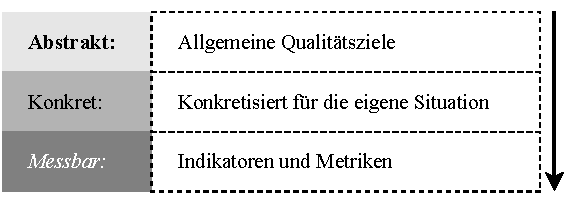
\includegraphics{contents/02_basics/res/quality_models.pdf}
    \caption{Aufbau eines Qualitätsmodells in drei Ebenen \cite[S. 34, ][]{schneider2012abenteuer}}
    \label{fig:basics_quality_models}
\end{figure}

\cite{schneider2012abenteuer}